\section{Technical Architecture}

The \glsxtrshort{cuinspace} telemetry system software will be composed of multiple modules:

\begin{enumerate}
    \setlength{\itemsep}{1pt}
    \setlength{\parskip}{0pt} \setlength{\parsep}{0pt}
    \item \texttt{controller}
    \item \texttt{fetcher}
    \item \texttt{packager}
    \item \texttt{broadcaster}
    \item \texttt{writer}
\end{enumerate}

\subsection{Architecture Diagrams}

The architecture for the \glsxtrshort{cuinspace} telemetry system is separated into two system designs:
\begin{enumerate}
    \setlength{\itemsep}{1pt}
    \setlength{\parskip}{0pt} \setlength{\parsep}{0pt}
    \item Critical functionality \hyperref[fig:crit-arc]{(Figure \ref{fig:crit-arc})}
    \item Non-critical functionality \hyperref[fig:non-crit-arc]{(Figure \ref{fig:non-crit-arc})}
\end{enumerate}

Critical functionality is required for a functional telemetry system in the 2023-2024 academic year. Non-critical
functionality can be postponed until the 2024-2025 academic year.

\begin{figure}[H]
    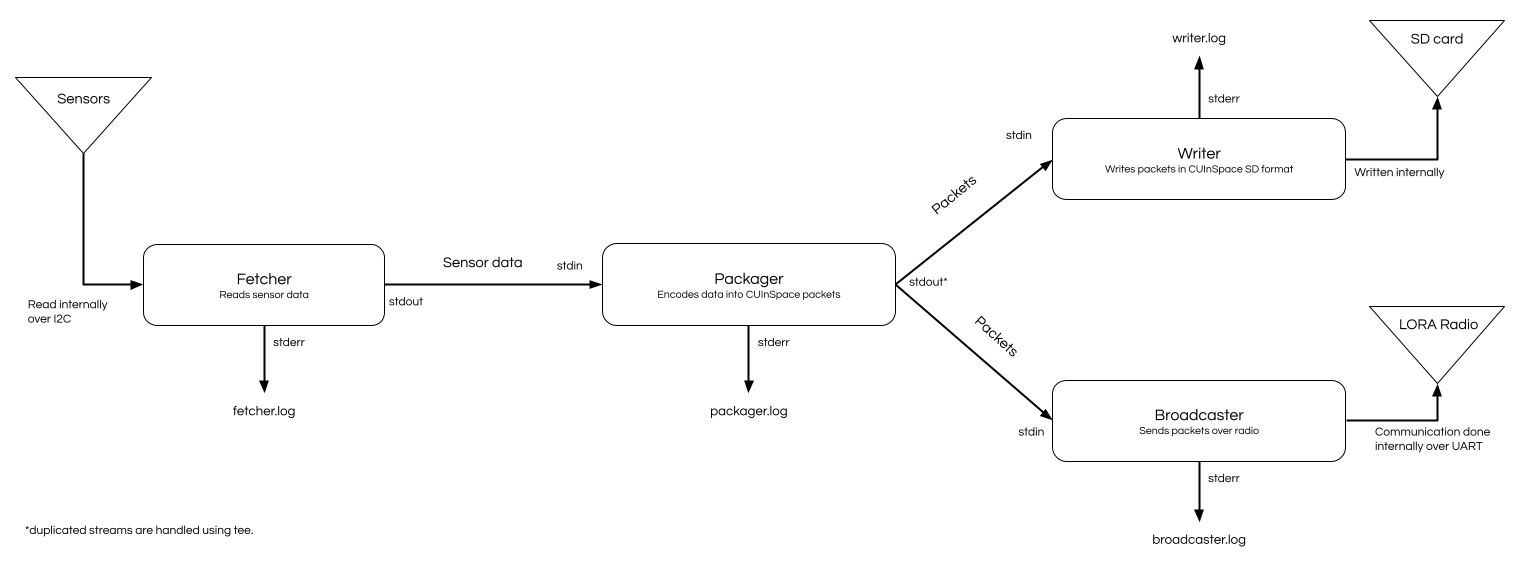
\includegraphics[width=\linewidth]{assets/critical-architecture.png}
    \caption{System diagram of the critical functionality for the telemetry system}
    \label{fig:crit-arc}
\end{figure}

\begin{figure}[H]
    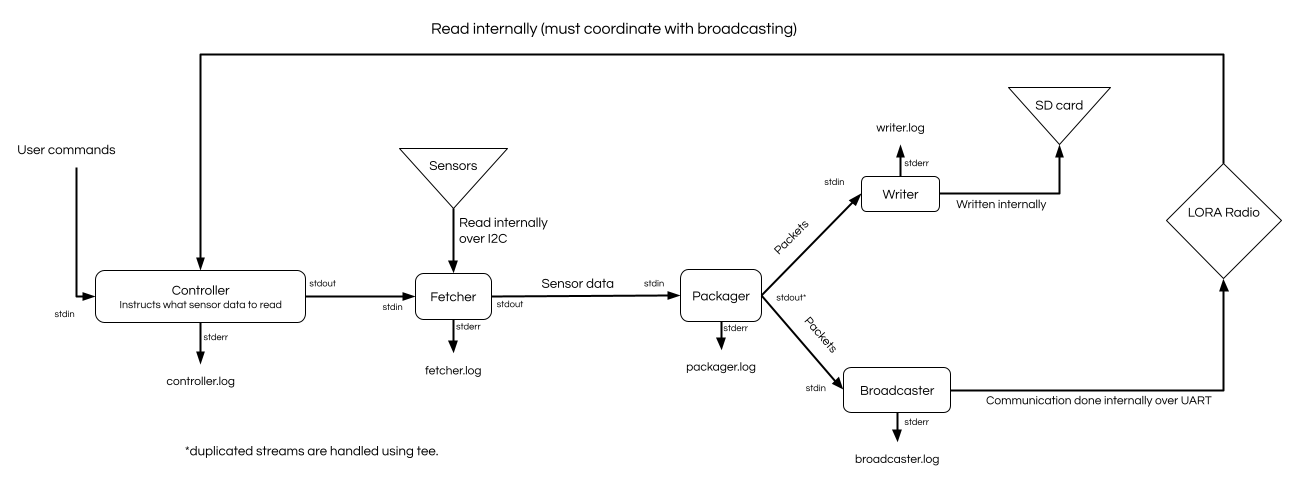
\includegraphics[width=\linewidth]{assets/non-critical-architecture.png}
    \caption{System diagram of the non-critical functionality for the telemetry system}
    \label{fig:non-crit-arc}
\end{figure}

\subsection{Modules} \label{s:modules}

Each module makes use of the \gls{unix} philosophy: do one task, and do it well. Modules are \glsxtrfull{posix}
compliant in order to be portable across other \glsxtrshort{posix} compliant \glsxtrshortpl{rtos}. As part of the
adoption of the \gls{unix} philosophy, each module will also expect their input in plain-text (where applicable) and
provide their output in plain text. This allows each module's output to be useful on its own as well as part of the
whole system, rather than being tailored for input into another module. Additionally, a plain-text output makes it
easier for developers to reason about and debug module output.

All of the modules are written in the C programming language, in order to make use of \gls{qnx}'s included C libraries.
This also facilitates \glsxtrshort{srad} development, as members in the engineering and computer science programs
become familiar with C programming early in their undergraduate degree.

All modules use \texttt{\gls{stdin}}, \texttt{\gls{stdout}} and \texttt{\gls{stderr}} for \glsxtrfull{ipc}. Error
messages and logs are sent to \texttt{\gls{stderr}} so that they can be easily separated from other program output and
redirected to a log file. Modules read their input from \texttt{\gls{stdin}} to be processed, and write their output to
\texttt{\gls{stdout}}. This allows for modules to be piped into each other easily. Modules will also be able to read
from a file or a \gls{fifo} in addition to \texttt{\gls{stdin}} for more control using output duplication with the
\gls{posixgls} \texttt{tee} command.

None of the libraries developed for use in the modules make assumptions about memory allocation, and instead accept
pre-allocated memory blocks to initialize with data. This allows modules to be portable to embedded systems with less
development overhead.

All modules are bundled with help text which can be displayed with the \texttt{use} command. The help text contains a
description of the module, its usage, example calls, and command line options and their default values.

All modules follow the gnu11 C standard. This standard was selected because it is a modern C standard which permits the
use of \gls{gnu} libraries (such as \texttt{getopt}, a library for \glsxtrshort{posix} compliant command line
interfaces).

\subsubsection{Controller}

\textbf{This module is not part of the critical functionality for the 2023-2024 \glsxtrshort{cuinspace} telemetry
    system.}

The \texttt{controller} module is responsible for receiving control commands from the ground station over
\glsxtrshort{lora} and providing them to \texttt{fetcher} for interpretation. The \glsxtrshort{cuinspace} packet format
specification describes control packets which allow the ground station to request only specific types of telemetry data
from the rocket telemetry system. \cite{telemetry-format} The \texttt{controller} module will read these control
packets from the \glsxtrshort{lora} RN2483 chip and provide them as plain-text instructions to the \texttt{fetcher}
module.

The \texttt{controller} module will also be able to generate signal reports and report the \glsxtrshort{lora} radio
settings for diagnostic information. It may later be modified to additionally take input from an interactive terminal
interface so that the telemetry system can be monitored and controlled by developers during testing, or via SSH from
the launch pad. The module will also have the ability to modify radio parameters in accordance with the control packets
it receives from the ground station.

\subsubsection{Fetcher}

The \texttt{fetcher} module is responsible for perpetually reading sensor data. It does so by repeatedly polling for
data from all the sensors on the \glsxtrshort{cuinspace} \glsxtrshort{srad} sensor board via an \glsxtrshort{i2c} bus.

The \texttt{fetcher} module will output sensor data in plain-text over \texttt{\gls{stdout}} so that it can be used as
a standalone module. Outputted sensor data will be annotated with its data type (altitude, temperature, etc.) and unit
of measurement (metres, degrees Celsius, etc.).

The \texttt{fetcher} module will be able to receive instructions to prioritize certain sensor data via
\texttt{\gls{stdin}}. It will also be able to accept configuration which specifies sensor addresses, sensor data types
(altitude, temperature, etc.) and commands for reading from the sensors in order to be configurable for different
\glsxtrshort{srad} sensor boards. This configuration may be provided via a configuration file or command line
arguments. It is possible that sensor board hardware will be developed to include an \glsxtrfull{eeprom} on the
\glsxtrshort{i2c} bus containing this configuration information. \textbf{This functionality is not part of the critical
    requirements for the 2023-2024 telemetry system}.

\subsubsection{Packager}

The \texttt{packager} module is responsible for packaging sensor data into the \glsxtrshort{cuinspace} telemetry packet
format. It requires an \gls{ham-radio} call sign provided via command line in order to sign all the packets that it
creates, as well as plain-text sensor data provided over \texttt{\gls{stdin}} or via a file. \texttt{packager} will
write the encoded radio packets to \texttt{\gls{stdout}} in plain-text hexadecimal digits.

\subsubsection{Broadcaster}

The \texttt{broadcaster} module is responsible for interfacing with the \glsxtrshort{lora} RN2483 radio chip over
\glsxtrshort{uart} to broadcast packets to the ground station. It accepts input in the form of plain-text hexadecimal
digits over \texttt{\gls{stdin}} (or a file), which it sends to the radio chip for transmission. Newline characters in
the input signify the end of a packet. \texttt{broadcaster} will also accept command line options for all of the
configurable radio parameters provided by the RN2483 chip, which it will use for transmission.

\subsubsection{Writer}

The \texttt{writer} module is responsible for writing \glsxtrshort{cuinspace} telemetry packets to an SD card using the
\glsxtrshort{cuinspace} SD card storage format. The SD storage format uses the packet format in its entirety, but adds
some additional information for locating data from different flights. \cite{sd-format}

\texttt{writer} will also accept its input in the form of plain-text hexadecimal digits, either via \texttt{\gls{stdin}}
or a file. The input to writer must be valid \glsxtrshort{cuinspace} packets, which is its primary difference from
\texttt{broadcaster}. This is because packet data plays a role in generating the SD card format.

\subsection{Build System}

The build system for all software modules will be implemented using \gls{make}. \Gls{make} was chosen because of its
simplicity and wide adoption across software projects, especially C projects. The command line utility is available for
Windows and \glsxtrshort{posix} operating systems, and a version of it is included with the \gls{qnx} build system for
consistency across machines.

The \gls{make} build system also integrates with \gls{qnx}'s existing build system to recursively compile and link the
provided libraries. \Gls{qnx}'s build system also allows automatic building of multiple executables for different
architectures with the addition of sub directories to the project directory. \cite{qnx-dir-structure} The build system
can also bundle executables with their help documentation for integration with the \texttt{use} command.
\cite{qnx-dir-structure}
